\documentclass[11pt]{article}

%--------------------------------------------------------------------
% Package Imports & Configuration
%--------------------------------------------------------------------
\usepackage[margin=1in]{geometry}          % Page margins
\usepackage[T1]{fontenc}                  % Output font encoding
\usepackage{lmodern}                      % Latin Modern for a modern look
\usepackage{hyperref}                     % Hyperlinks in PDF
\usepackage{xcolor}                       % Colors for text, boxes, and TikZ
\usepackage{tikz}                         % TikZ for diagrams
\usetikzlibrary{shapes,arrows,positioning,calc,arrows.meta,shapes.misc}
  % Removed 'cloud' library since it doesn't exist in all distributions.
  % 'shapes.misc' includes the 'cloud' shape.

% We use minted for highlighted code. Requires --shell-escape to compile.
\usepackage{minted}

% A bit of extra vertical space between paragraphs for readability:
\setlength{\parskip}{6pt}
\setlength{\parindent}{0pt}

%--------------------------------------------------------------------
% Custom TikZ Styles
%--------------------------------------------------------------------
\tikzset{
  serviceBox/.style={
    rectangle,
    rounded corners,
    draw=black,
    fill=blue!10,
    text width=3.2cm,
    minimum height=1.3cm,
    align=center
  },
  arrowLine/.style={
    -{Latex[length=3mm,width=2mm]},
    thick
  },
  cloudService/.style={
    cloud,
    draw=black,
    fill=blue!10,
    cloud puffs=15,
    cloud puff arc=120,
    aspect=2,
    minimum width=2.8cm,
    align=center
  },
  database/.style={
    cylinder,
    cylinder uses custom fill,
    cylinder body fill=blue!10,
    cylinder end fill=blue!10,
    draw=black,
    shape aspect=0.7,
    minimum height=2.2cm,
    minimum width=1.4cm,
    align=center
  },
  userFigure/.style={
    draw,
    fill=green!10,
    rounded corners,
    text width=2.8cm,
    minimum height=1.2cm,
    align=center
  }
}

%--------------------------------------------------------------------
% Title and Meta Info
%--------------------------------------------------------------------
\title{\textbf{A Simple, Visual Introduction to AWS}\\ \large (Improved Edition)}
\author{}
\date{\today}

\begin{document}
\maketitle

\tableofcontents
\vspace{1cm}

%--------------------------------------------------------------------
% INTRO
%--------------------------------------------------------------------
\section*{Introduction}
\addcontentsline{toc}{section}{Introduction}

This updated document aims to give newcomers an easy-to-follow, visually guided introduction to \textbf{Amazon Web Services (AWS)}. Whether you're building a small personal project or diving into large-scale deployments, AWS offers a wide range of services to help you succeed. This guide focuses on:

\begin{itemize}
    \item \textbf{What AWS is and why it matters}
    \item \textbf{Common use cases in the real world}
    \item \textbf{Step-by-step learning projects}
    \item \textbf{Many diagrams to illustrate core concepts}
\end{itemize}

\clearpage

%--------------------------------------------------------------------
% 1. WHAT IS AWS?
%--------------------------------------------------------------------
\section{What is AWS?}

\subsection{Definition}
\textbf{Amazon Web Services (AWS)} is a cloud computing platform that lets you:

\begin{itemize}
    \item Rent computing resources on-demand
    \item Store, process, and analyze data
    \item Host and scale applications globally
\end{itemize}

\vspace{2pt}
\textbf{Key Benefits:}
\begin{itemize}
    \item \textbf{Pay-As-You-Go}: Only pay for the resources you actually use.
    \item \textbf{Scalability}: Effortlessly adjust capacity based on real-time traffic.
    \item \textbf{Global Infrastructure}: Deploy and deliver content across multiple regions worldwide.
\end{itemize}

\subsection{Service Categories}
AWS is large, but it helps to see services grouped by functionality:

\begin{itemize}
    \item \textbf{Compute}: EC2 (virtual servers), Lambda (serverless)
    \item \textbf{Storage}: S3 (object storage), EBS (block storage)
    \item \textbf{Database}: RDS (relational), DynamoDB (NoSQL)
    \item \textbf{Networking}: VPC, CloudFront (CDN)
    \item \textbf{Analytics}: Kinesis, Athena
    \item \textbf{Machine Learning}: SageMaker
\end{itemize}

\subsection{High-Level Visualization}

\begin{center}
    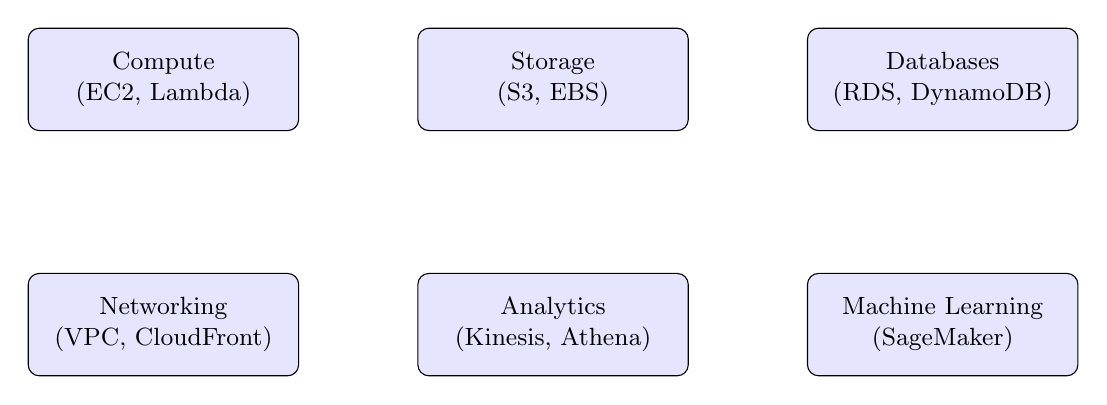
\begin{tikzpicture}[
            node distance=2.3cm,
            every node/.style={font=\small}
        ]
        \node[serviceBox] (compute) {Compute\\(EC2, Lambda)};
        \node[serviceBox, right=1.5cm of compute] (storage) {Storage\\(S3, EBS)};
        \node[serviceBox, right=1.5cm of storage] (db) {Databases\\(RDS, DynamoDB)};

        \node[serviceBox, below=1.8cm of compute] (network) {Networking\\(VPC, CloudFront)};
        \node[serviceBox, right=1.5cm of network] (analytics) {Analytics\\(Kinesis, Athena)};
        \node[serviceBox, right=1.5cm of analytics] (ml) {Machine Learning\\(SageMaker)};

    \end{tikzpicture}
\end{center}

\clearpage

%--------------------------------------------------------------------
% 2. HOW COMPANIES USE AWS
%--------------------------------------------------------------------
\section{How Companies Use AWS}

\subsection{Web Hosting}
Many companies host their websites or web applications on AWS. Options range from:
\begin{itemize}
    \item \textbf{Static sites}: Simple S3 + CloudFront setup
    \item \textbf{Dynamic sites}: EC2-based servers or container services (ECS, EKS)
\end{itemize}

\subsubsection{Example: Static Hosting with S3 and CloudFront}

\begin{center}
    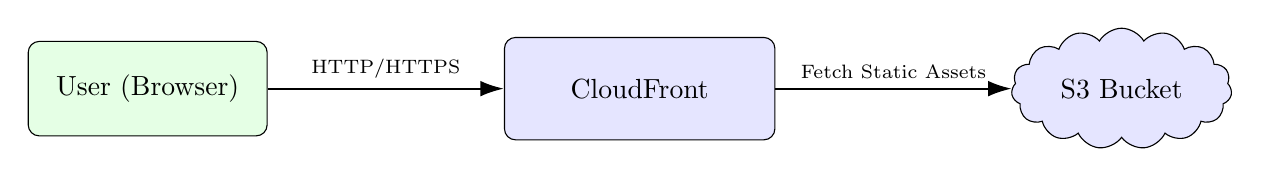
\begin{tikzpicture}[node distance=2.5cm]
        \node[userFigure] (user) {User (Browser)};
        \node[serviceBox, right=3.0cm of user] (cloudfront) {CloudFront};
        \node[cloudService, right=3.0cm of cloudfront] (s3) {S3 Bucket};

        \draw[arrowLine] (user) -- node[above]{\scriptsize HTTP/HTTPS} (cloudfront);
        \draw[arrowLine] (cloudfront) -- node[above]{\scriptsize Fetch Static Assets} (s3);

    \end{tikzpicture}
\end{center}

\subsection{Data Storage and Backup}
Many organizations use \textbf{Amazon S3} for storing large files, media, or backups. It’s highly durable (99.999999999\% durability) and integrates well with other AWS services.

\begin{center}
    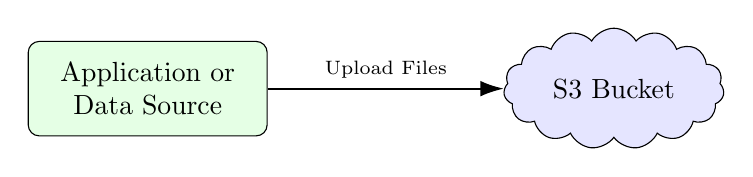
\begin{tikzpicture}[node distance=2.2cm]
        \node[userFigure] (app) {Application or Data Source};
        \node[cloudService, right=3cm of app] (s3) {S3 Bucket};

        \draw[arrowLine] (app) -- node[above]{\scriptsize Upload Files} (s3);
    \end{tikzpicture}
\end{center}

\subsection{Application Development and Deployment}
AWS supports various application architectures, from traditional server-based (EC2) to fully \textbf{serverless} (Lambda). Developers often use:
\begin{itemize}
    \item \textbf{API Gateway} to create REST or WebSocket APIs
    \item \textbf{Lambda} to run code without provisioning servers
    \item \textbf{DynamoDB} or \textbf{RDS} as the database layer
\end{itemize}

\begin{center}
    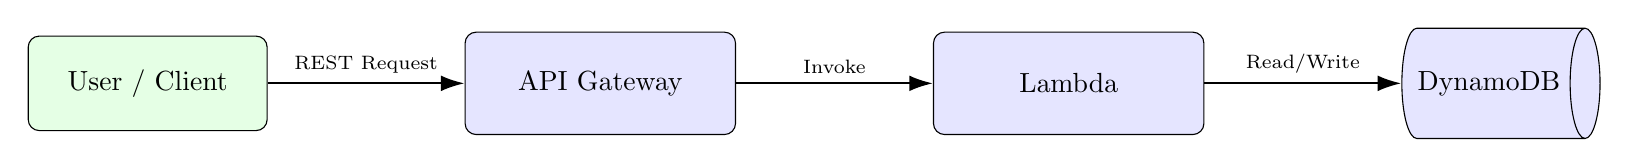
\begin{tikzpicture}[node distance=2.3cm]
        \node[userFigure] (client) {User / Client};
        \node[serviceBox, right=2.5cm of client] (apiGW) {API Gateway};
        \node[serviceBox, right=2.5cm of apiGW] (lambda) {Lambda};
        \node[database, right=2.5cm of lambda] (ddb) {DynamoDB};

        \draw[arrowLine] (client) -- node[above]{\scriptsize REST Request} (apiGW);
        \draw[arrowLine] (apiGW) -- node[above]{\scriptsize Invoke} (lambda);
        \draw[arrowLine] (lambda) -- node[above]{\scriptsize Read/Write} (ddb);
    \end{tikzpicture}
\end{center}

\subsection{Machine Learning}
AWS offers \textbf{SageMaker} to simplify building, training, and deploying ML models. Common workflow:
\begin{itemize}
    \item Store dataset in S3
    \item Train model in SageMaker
    \item Deploy model endpoint
\end{itemize}

\subsection{Analytics}
Analyze large volumes of data or real-time streams:
\begin{itemize}
    \item \textbf{Kinesis} for real-time data ingestion
    \item \textbf{Athena} to query S3 data with standard SQL
\end{itemize}

\clearpage

%--------------------------------------------------------------------
% 3. HOW YOU CAN USE AWS
%--------------------------------------------------------------------
\section{How You Can Use AWS}

\subsection{Starting Small}
Even beginners can build:
\begin{itemize}
    \item \textbf{Static portfolio site}: Hosted on S3 + CloudFront
    \item \textbf{File processor}: Upload an image to S3, resize it using Lambda, and store the result
\end{itemize}

\subsection{Workflow Automation}
AWS excels at \textbf{event-driven} workflows:
\begin{center}
    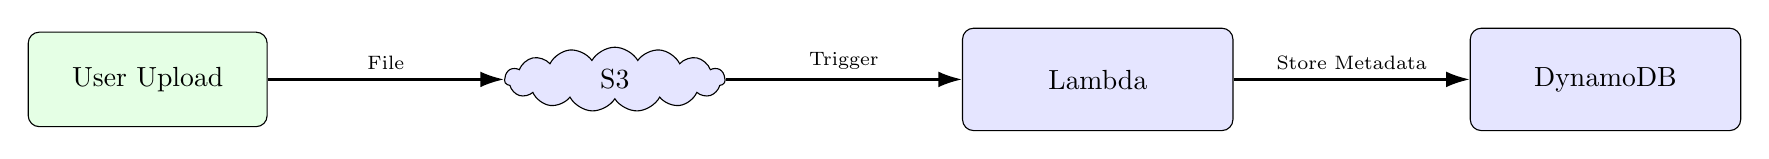
\begin{tikzpicture}[node distance=3.0cm]
        \node[userFigure] (upload) {User Upload};
        \node[cloudService, right=3cm of upload] (s3) {S3};
        \node[serviceBox, right=3cm of s3] (lambda) {Lambda};
        \node[serviceBox, right=3cm of lambda] (ddb) {DynamoDB};

        \draw[arrowLine] (upload) -- node[above]{\scriptsize File} (s3);
        \draw[arrowLine] (s3) -- node[above]{\scriptsize Trigger} (lambda);
        \draw[arrowLine] (lambda) -- node[above]{\scriptsize Store Metadata} (ddb);
    \end{tikzpicture}
\end{center}

\subsection{Monitoring and Logging}
\textbf{CloudWatch} collects logs from your AWS resources, provides metrics, and can trigger alarms or scaling actions when thresholds are met.

\begin{center}
    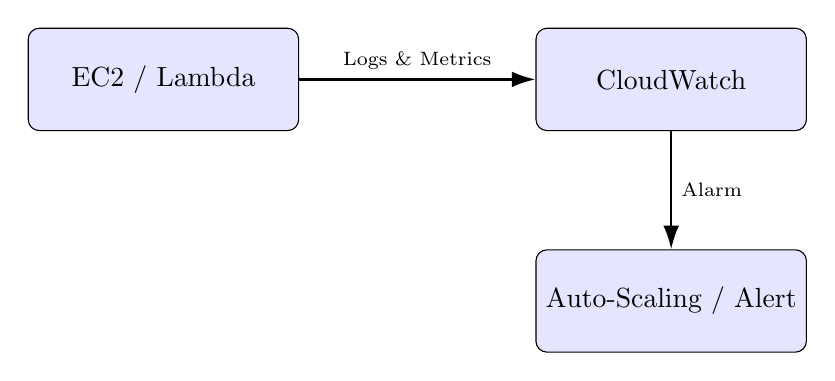
\begin{tikzpicture}[node distance=2.2cm]
        \node[serviceBox] (resource) {EC2 / Lambda};
        \node[serviceBox, right=3cm of resource] (cw) {CloudWatch};

        \draw[arrowLine] (resource) -- node[above]{\scriptsize Logs \& Metrics} (cw);

        \node[serviceBox, below=1.5cm of cw] (scale) {Auto-Scaling / Alert};
        \draw[arrowLine] (cw) -- node[right]{\scriptsize Alarm} (scale);
    \end{tikzpicture}
\end{center}

\clearpage

%--------------------------------------------------------------------
% 4. KEY AWS SERVICES
%--------------------------------------------------------------------
\section{Key AWS Services (Simplified Overview)}

\subsection{S3 (Object Storage)}
A scalable, secure, and cost-effective way to store large quantities of files.
\begin{center}
    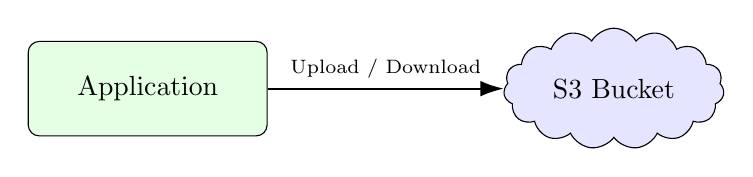
\begin{tikzpicture}[node distance=2.5cm]
        \node[userFigure] (source) {Application};
        \node[cloudService, right=3cm of source] (s3b) {S3 Bucket};

        \draw[arrowLine] (source) -- node[above]{\scriptsize Upload / Download} (s3b);
    \end{tikzpicture}
\end{center}

\subsection{Lambda (Serverless Compute)}
Write code functions that respond to events (e.g., S3 uploads, API Gateway calls). No need to manage servers.

\begin{minted}[fontsize=\small, frame=single]{python}
def ProcessFile(event, context):
    S3_BUCKET_NAME = "my-bucket"
    fileKey = event["Records"][0]["s3"]["object"]["key"]

    # ... do something interesting here ...

    return {
        "statusCode": 200,
        "body": "Processing complete"
    }
\end{minted}

\subsection{DynamoDB (NoSQL)}
Key-value store optimized for performance and scalability. Excellent choice for user profiles, session data, or IoT data.

\subsection{EC2 (Virtual Servers)}
Allows you to rent and configure virtual machines. Ideal if you need complete control over the OS and software environment.

\subsection{CloudFront (CDN)}
A global content delivery network that caches and delivers content (static or dynamic) from edge locations near your users.

\clearpage

%--------------------------------------------------------------------
% 5. SUGGESTED PROJECTS
%--------------------------------------------------------------------
\section{Suggested Projects for Hands-On Learning}

\subsection{Beginner Level}
\textbf{1. Static Website}
\begin{itemize}
    \item Host a personal resume or portfolio on S3
    \item Use CloudFront to speed up global delivery
\end{itemize}

\textbf{2. File Processor with Lambda and S3}
\begin{itemize}
    \item Upload an image to S3
    \item Lambda automatically resizes/optimizes the image
    \item Outputs to another S3 bucket or the same bucket
\end{itemize}

\subsection{Intermediate Level}
\textbf{1. Web App with EC2, RDS, and S3}
\begin{itemize}
    \item EC2: runs your backend
    \item RDS: relational database
    \item S3: static images or media
\end{itemize}

\textbf{2. Serverless API (API Gateway + Lambda + DynamoDB)}
Create a REST or GraphQL API. Lambda handles business logic; DynamoDB stores the data.

\subsection{Advanced Level}
\textbf{1. Real-Time Data (Kinesis + Lambda + DynamoDB)}
\begin{itemize}
    \item Kinesis streams incoming data
    \item Lambda processes records in near real time
    \item DynamoDB stores aggregated or processed data
\end{itemize}

\textbf{2. Machine Learning (SageMaker + S3 + Lambda)}
\begin{itemize}
    \item S3 for training data
    \item SageMaker to train and host the model
    \item Lambda or a web app calls the deployed model endpoint
\end{itemize}

\begin{center}
    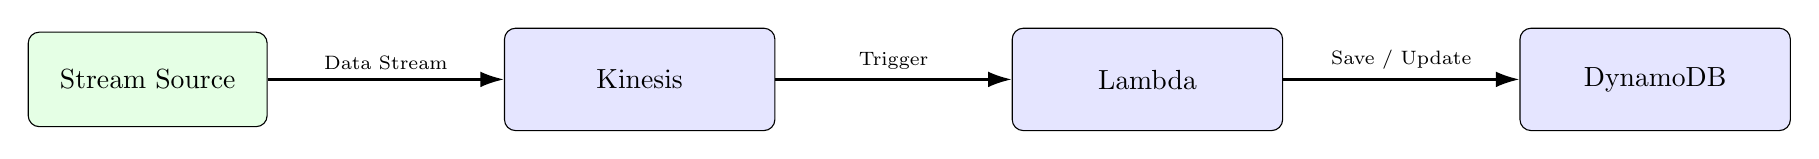
\begin{tikzpicture}[node distance=2.5cm]
        \node[userFigure] (source) {Stream Source};
        \node[serviceBox, right=3cm of source] (kinesis) {Kinesis};
        \node[serviceBox, right=3cm of kinesis] (lambda) {Lambda};
        \node[serviceBox, right=3cm of lambda] (ddb) {DynamoDB};

        \draw[arrowLine] (source) -- node[above]{\scriptsize Data Stream} (kinesis);
        \draw[arrowLine] (kinesis) -- node[above]{\scriptsize Trigger} (lambda);
        \draw[arrowLine] (lambda) -- node[above]{\scriptsize Save / Update} (ddb);
    \end{tikzpicture}
\end{center}

\clearpage

%--------------------------------------------------------------------
% 6. ADDITIONAL VISUALIZATIONS
%--------------------------------------------------------------------
\section{Additional Visualizations}

\subsection{Application Architecture (Serverless Example)}
\begin{center}
    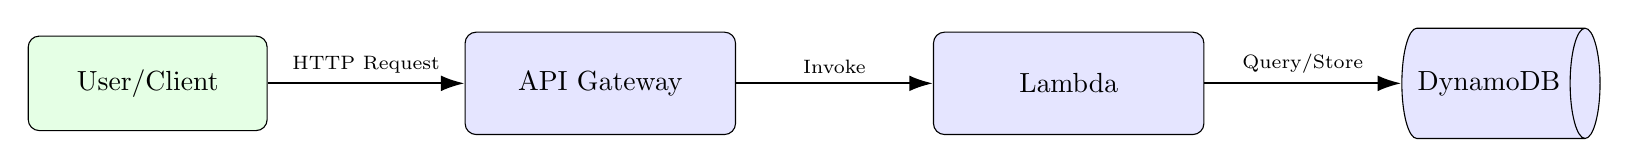
\begin{tikzpicture}[node distance=2cm]
        \node[userFigure] (user) {User/Client};
        \node[serviceBox, right=2.5cm of user] (apiGW) {API Gateway};
        \node[serviceBox, right=2.5cm of apiGW] (lambda) {Lambda};
        \node[database, right=2.5cm of lambda] (database) {DynamoDB};

        \draw[arrowLine] (user) -- node[above]{\scriptsize HTTP Request} (apiGW);
        \draw[arrowLine] (apiGW) -- node[above]{\scriptsize Invoke} (lambda);
        \draw[arrowLine] (lambda) -- node[above]{\scriptsize Query/Store} (database);
    \end{tikzpicture}
\end{center}

\subsection{Monitoring and Alerting Loop}
\begin{center}
    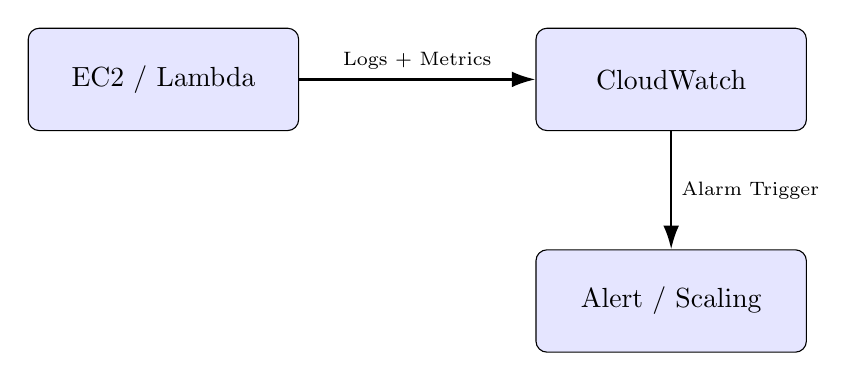
\begin{tikzpicture}[node distance=2.3cm]
        \node[serviceBox] (instances) {EC2 / Lambda};
        \node[serviceBox, right=3cm of instances] (cw) {CloudWatch};

        \draw[arrowLine] (instances) -- node[above]{\scriptsize Logs + Metrics} (cw);

        \node[serviceBox, below=1.5cm of cw] (alert) {Alert / Scaling};
        \draw[arrowLine] (cw) -- node[right]{\scriptsize Alarm Trigger} (alert);

    \end{tikzpicture}
\end{center}

\clearpage

%--------------------------------------------------------------------
% 7. LEARNING PATH
%--------------------------------------------------------------------
\section{Learning Path}

\subsection{1. Foundation}
Focus on:
\begin{itemize}
    \item S3 (basic storage)
    \item Lambda (serverless compute)
    \item DynamoDB (simple NoSQL)
\end{itemize}
Build small automation or workflow projects to get comfortable with the AWS console and basic configurations.

\subsection{2. Intermediate Services}
Once comfortable, expand:
\begin{itemize}
    \item \textbf{API Gateway} for building APIs
    \item \textbf{RDS} for relational data
    \item \textbf{EC2} for custom environments
\end{itemize}

\subsection{3. Advanced Tools}
Tackle big-data or specialized domains:
\begin{itemize}
    \item \textbf{Kinesis} for real-time event streaming
    \item \textbf{SageMaker} for machine learning
    \item \textbf{Redshift} or \textbf{Athena} for analytics
\end{itemize}

\begin{center}
    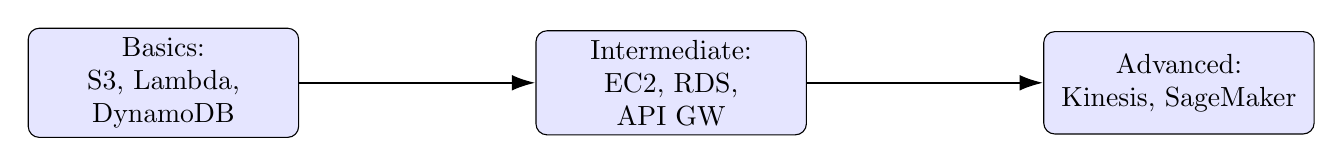
\begin{tikzpicture}[node distance=2.5cm]
        \node[serviceBox] (basic) {Basics:\\S3, Lambda, DynamoDB};
        \node[serviceBox, right=3cm of basic] (inter) {Intermediate:\\EC2, RDS, API GW};
        \node[serviceBox, right=3cm of inter] (advanced) {Advanced:\\Kinesis, SageMaker};

        \draw[arrowLine] (basic) -- (inter);
        \draw[arrowLine] (inter) -- (advanced);
    \end{tikzpicture}
\end{center}

\clearpage

%--------------------------------------------------------------------
% CONCLUSION
%--------------------------------------------------------------------
\section*{Conclusion}
\addcontentsline{toc}{section}{Conclusion}

We’ve covered the basics of \textbf{AWS} in a simple, visually guided way. By starting with fundamental services like S3, Lambda, and DynamoDB, you can quickly grasp the core principles of the AWS ecosystem. Then you can incrementally add services---EC2, RDS, API Gateway---to handle more complex or performance-intensive applications. Eventually, you can move on to real-time data processing (Kinesis), large-scale analytics (Redshift, Athena), and machine learning (SageMaker).

Throughout this journey:
\begin{itemize}
    \item Keep experimenting with small, hands-on projects.
    \item Use the \textbf{AWS Free Tier} to control costs.
    \item Refer to official \href{https://aws.amazon.com/documentation/}{AWS Documentation} for deeper detail.
\end{itemize}

\textbf{Happy Building!}

\end{document}
